\documentclass[12pt]{article}
\usepackage[spanish]{babel}
\usepackage{csquotes}
\usepackage{amsmath}
\usepackage{graphicx}
\usepackage{float}
\usepackage{apacite} % Para citas APA
\usepackage{caption}
\usepackage{longtable} % Para tablas largas
\usepackage[letterpaper,top=2cm,bottom=2cm,left=1.5cm,right=1.5cm]{geometry}
\usepackage{fancyhdr} % Paquete para encabezado y pie de página

\pagestyle{fancy}
\fancyhf{} % Limpia encabezados y pies de página por defecto

% Configuración del encabezado
\fancyhead[L]{Universidad de Bolívar} % Encabezado izquierdo
\fancyhead[C]{} % Encabezado central vacío
\fancyhead[R]{Realidad Nacional y Diversidad Cultural} % Encabezado derecho

% Configuración del pie de página
\fancyfoot[C]{\thepage} % Pie de página central con el número de página

% Configuración especial para la primera página
% \fancypagestyle{firstpage}{
%   \fancyhf{}
%   \fancyhead[C]{Universidad de Bolívar} % Encabezado centrado en la primera página
%   \fancyfoot[C]{\thepage} % Pie de página centrado con número de página
% }

\title{Funciones y responsabilidades de los Gobiernos Autónomos Descentralizados}
\author{Ariel Alejandro Calderón}
\date{\today}

\begin{document}

\maketitle

\section{Introducción}

Los Gobiernos Autónomos Descentralizados (GADs) desempeñan un papel fundamental en la estructura administrativa de varios países, particularmente en aquellos con sistemas federales o descentralizados. La descentralización implica que estas entidades gubernamentales tienen responsabilidades específicas en la administración pública que permiten un desarrollo más equitativo y eficaz de sus jurisdicciones. Según \citeA{sen2010}, la autonomía de los GADs fomenta la participación ciudadana y la eficiencia administrativa. Este ensayo explora las funciones y responsabilidades principales de los GADs, basándose en diversas fuentes científicas y normativas.

\begin{figure}[H]
    \centering
    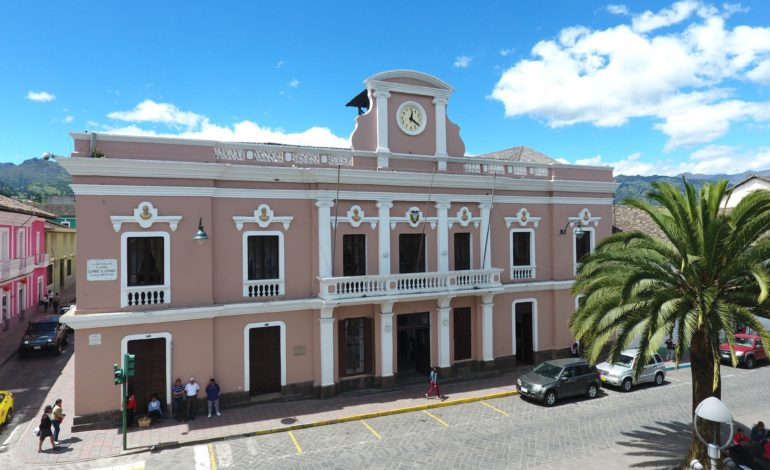
\includegraphics[width=0.5\textwidth]{./public/g1.jpg}
    % \caption{Palacio Municipal de Guaranda (imagen desde la Alcaldía de Guaranda)}
    \label{fig:desarrollo}
\end{figure}
\begin{center}
    \text{\cite{web2024}}
\end{center}
\section{Funciones y Responsabilidades de los GADs}

\begin{figure}[H]
    \centering
    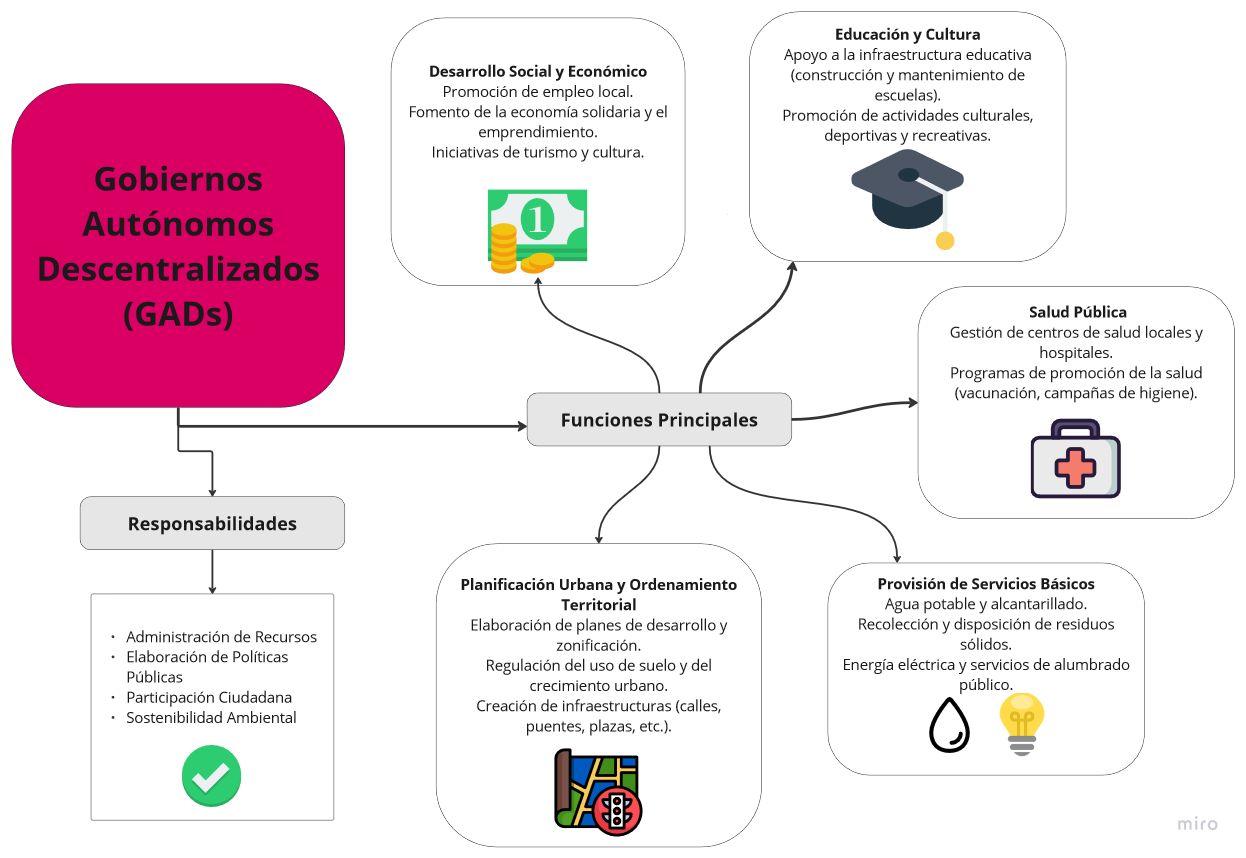
\includegraphics[width=1\textwidth]{./public/g2.png}
    \caption{Mapa mental}
    \label{fig: mapa mental}
\end{figure}


\section{Conclusión}

En conclusión, los Gobiernos Autónomos Descentralizados son cruciales para el desarrollo de las comunidades, ya que gestionan recursos y servicios que afectan directamente a la calidad de vida de los ciudadanos. La descentralización fomenta una mayor participación ciudadana, permite una administración más eficiente y cercana a las necesidades locales. \cite{pichincha2017}

\newpage

\bibliographystyle{apacite}
\bibliography{bibliografia}

\end{document}
